\subsection{Kartesische Produkte von Graphen}
In diesem Teil zeigen wir, was im Bezug auf die Anzahl der Spannbäume geschieht, wenn man das kartesische Produkt von Graphen bildet.\\
Das kartesische Produkt $G_1\times G_2$ zweier Graphen $G1=(V_1,E_1)$ und $G2=(V_2,E_2)$ bezeichnet dabei den Graphen mit Knotenmenge $V_1\times V_2$ und Kantenmenge $(E_1\times V_2)\cup(V_1\times E_2)$, wobei zwei Knoten $(u_1,u_2), (v_1,v_2) \in (V_1\times V_2)$ genau dann in $G_1\times G_2$ benachbart sind, wenn entweder $u_1=v_1$ in $G_1$ oder $u_2=v_2$ in $G_2$ ist.\\
\todo[inline, color=yellow]{Ich werde wahrscheinlich ein/zwei Beispiele davon zeigen, z.B. Lattice-Graph, aber nicht mehr, weil das im Grund genommen einfach nur Rechnungen sind und das Matrix-Tree-Theorem nicht mehr als solches angewendet wird, sondern nur über den Satz unten(passt das?)---Antwort:JA->warmup-kapitel}
\todo[inline, color=yellow]{Vielleicht ist es sinnvoll ein weiteres Kapitel mit einfachen Graphen wie Kreis-Graphen, Pfad-Graphen,etc. zu machen, dann könnte man sich in diesem Kapitel fast alle Rechnungen  ersparen und nur ein/zwei Beispiele geben, was man daraus "basteln" kann (Gute Idee?)---Antwort:JA}
\begin{Tms}
 Sei $G$ ein Graph mit $m$ Knoten und Eigenwerten $\mu_1(G),..,\mu_m(G)$ und $H$ ein Graph mit $n$ Knoten und Eigenwerten $\mu_1(H),..,\mu_n(H)$. \\
% Dann sind die Eigenwerte des kartesischen Produkts $G \times H$ genau $\mu_i(G)+\mu_j(H)$ mit $i \in \{ 1,..,m\}, j \in \{ 1,..,n\}$.
Dann hat der Graph $G \times H$ genau
\begin{equation}
\frac{1}{nm}\displaystyle\prod_{i,j}(\mu_i(G)+\mu_j(H))1_{\{\mu_i(G)+\mu_j(H)\neq0\}}
\end{equation}
Spannbäume.
\end{Tms}
\textbf{Beweis:}\\
Für diesen Beweis werden wir die Gestalt der Laplacematrix von $G \times H$ ausnutzen und dann mithilfe der linearen Algebra Aussagen über die Eigenwerte treffen.\\
Wir beobachten, dass die Laplacematrix von $G\times H$ die Kroneckersumme der Laplacematrizen von $G$ und $H$ ist.\\
Aus der linearen Algebra wissen wir nun, dass die Eigenwerte der Kroneckersumme $L(G) \oplus L(H)$ genau $\mu_i(G)+\mu_j(H)$ mit $i \in \{ 1,..,m\}, j \in \{ 1,..,n\}$ sind.\\
Mit Kirchhoffs Matrix-Tree-Theorem folgt nun
\begin{equation}
 \mathit{k}(G \times H) = \frac{1}{nm}\displaystyle\prod_{i,j}(\mu_i(G)+\mu_j(H))1_{\{\mu_i(G)+\mu_j(H)\neq0\}}
\end{equation}
Damit ist unser Satz bewiesen.
\begin{flushright} $\Box$ \end{flushright} 
\todo[inline]{Beweis ganz sauber fertigmachen, evtl. Quelle in der man was über ide Kroneckersumme nachlesen kann}
Als erstes, sehr anschauliches Beispiel betrachten wir Zylinder-Graphen $C_{m,n}$;
diese sind das kartesische Produkt eines Pfad-Graphen $P_m$ mit einem Kreisgraphen $C_n$.\\
In der Abbildung ~\ref{c8xp3} sehen wir den Zylinder-Graphen $C_{3,8}$.
\begin{figure}[H]
  \centering
 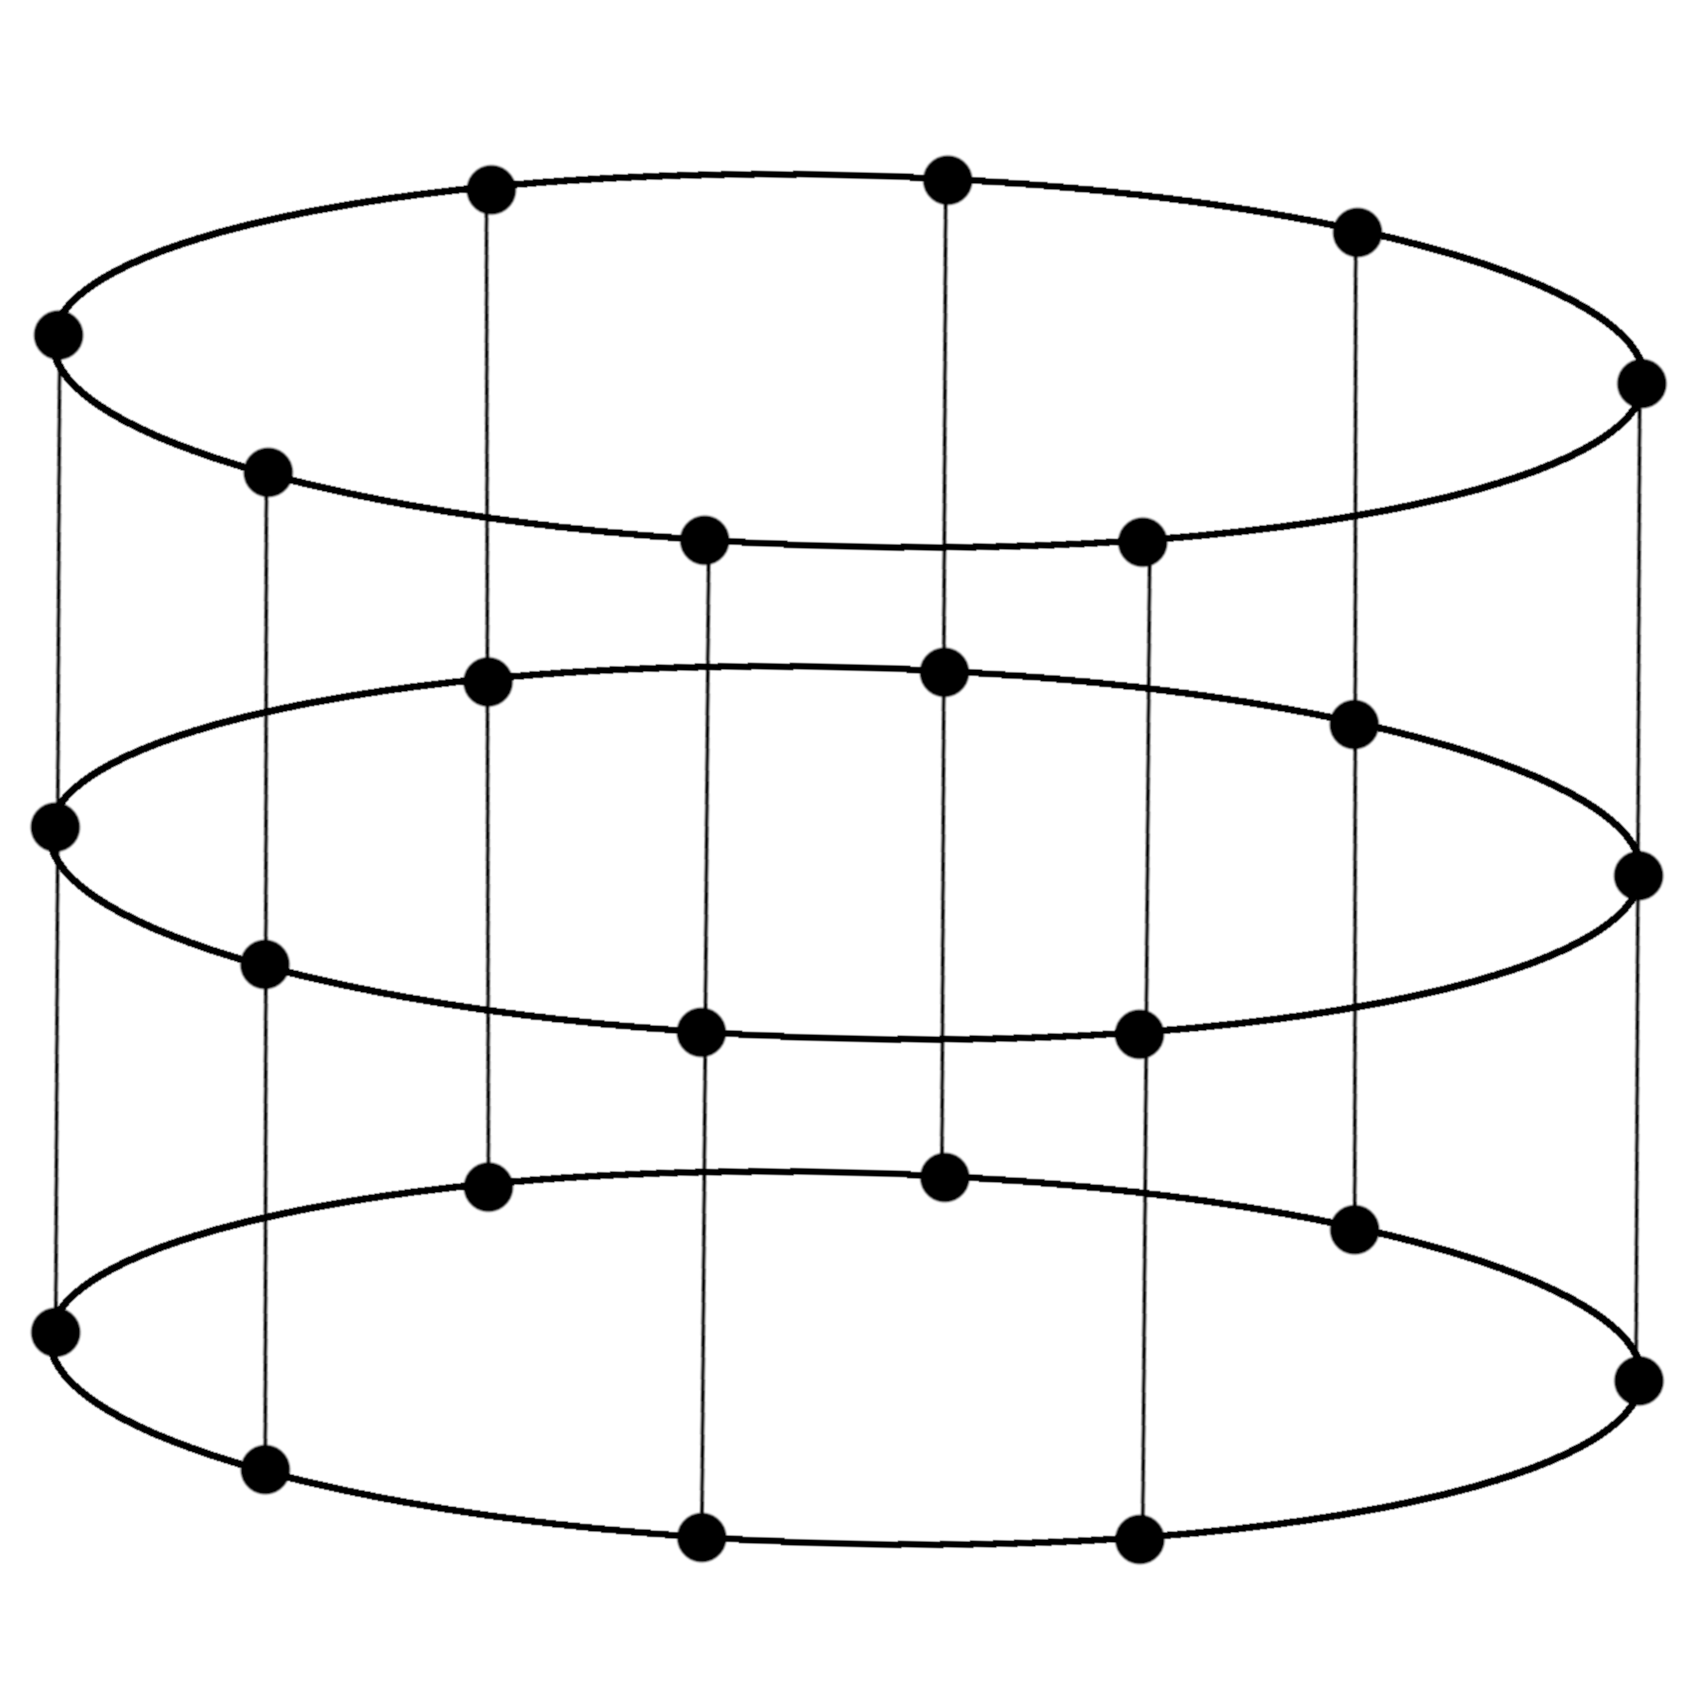
\includegraphics[width=0.25\textwidth]{c8xp3.png}
 \caption{$C_{3,8}$}
 \label{c8xp3} %caption vor label unbedingt
\end{figure}
\begin{Bsps}[Zylinder-Graph]
Blablablablabla\\
Blablablablabla
\end{Bsps}
Unser zweites Beispiel sind kartesische Produkte zweier Kreis-Graphen $C_m,C_n$; Man nennt diese dann auch Torus-Graphen, kurz $T_{m,n}$. Hier sehen wir so einen Graphen:
\begin{figure}[H]
  \centering
 %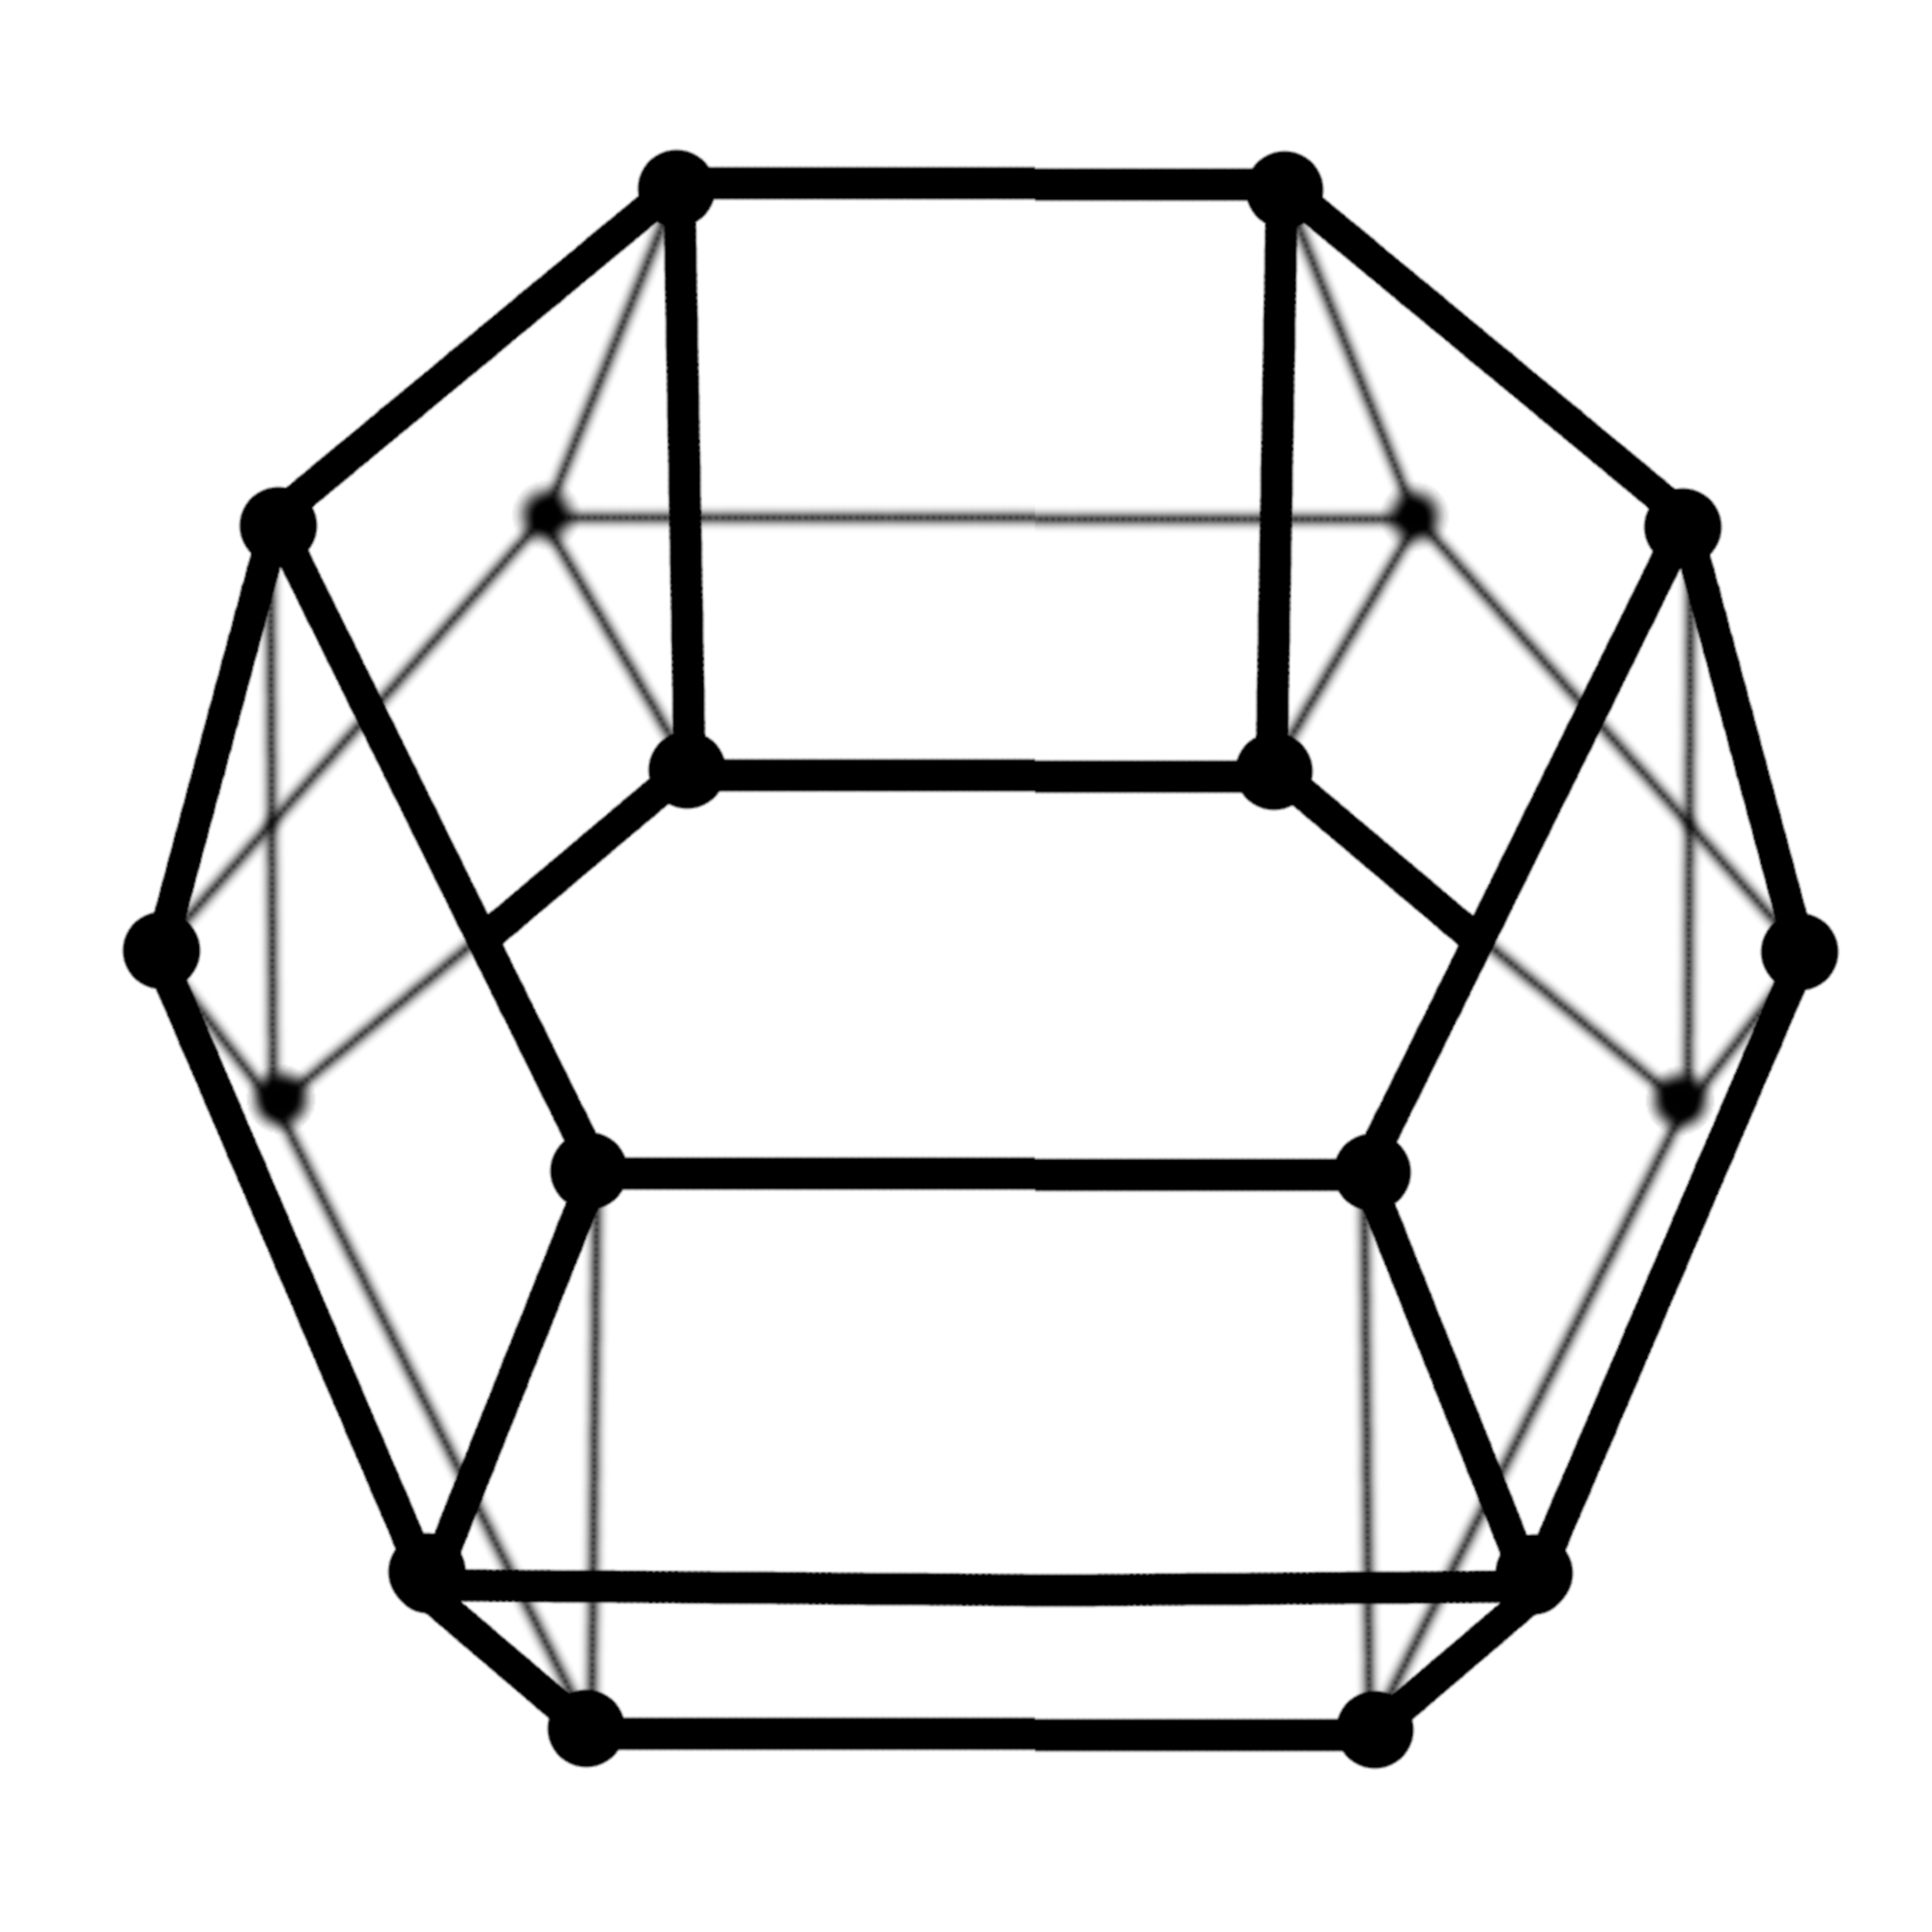
\includegraphics[width=0.25\textwidth]{C3xC6.png}
 %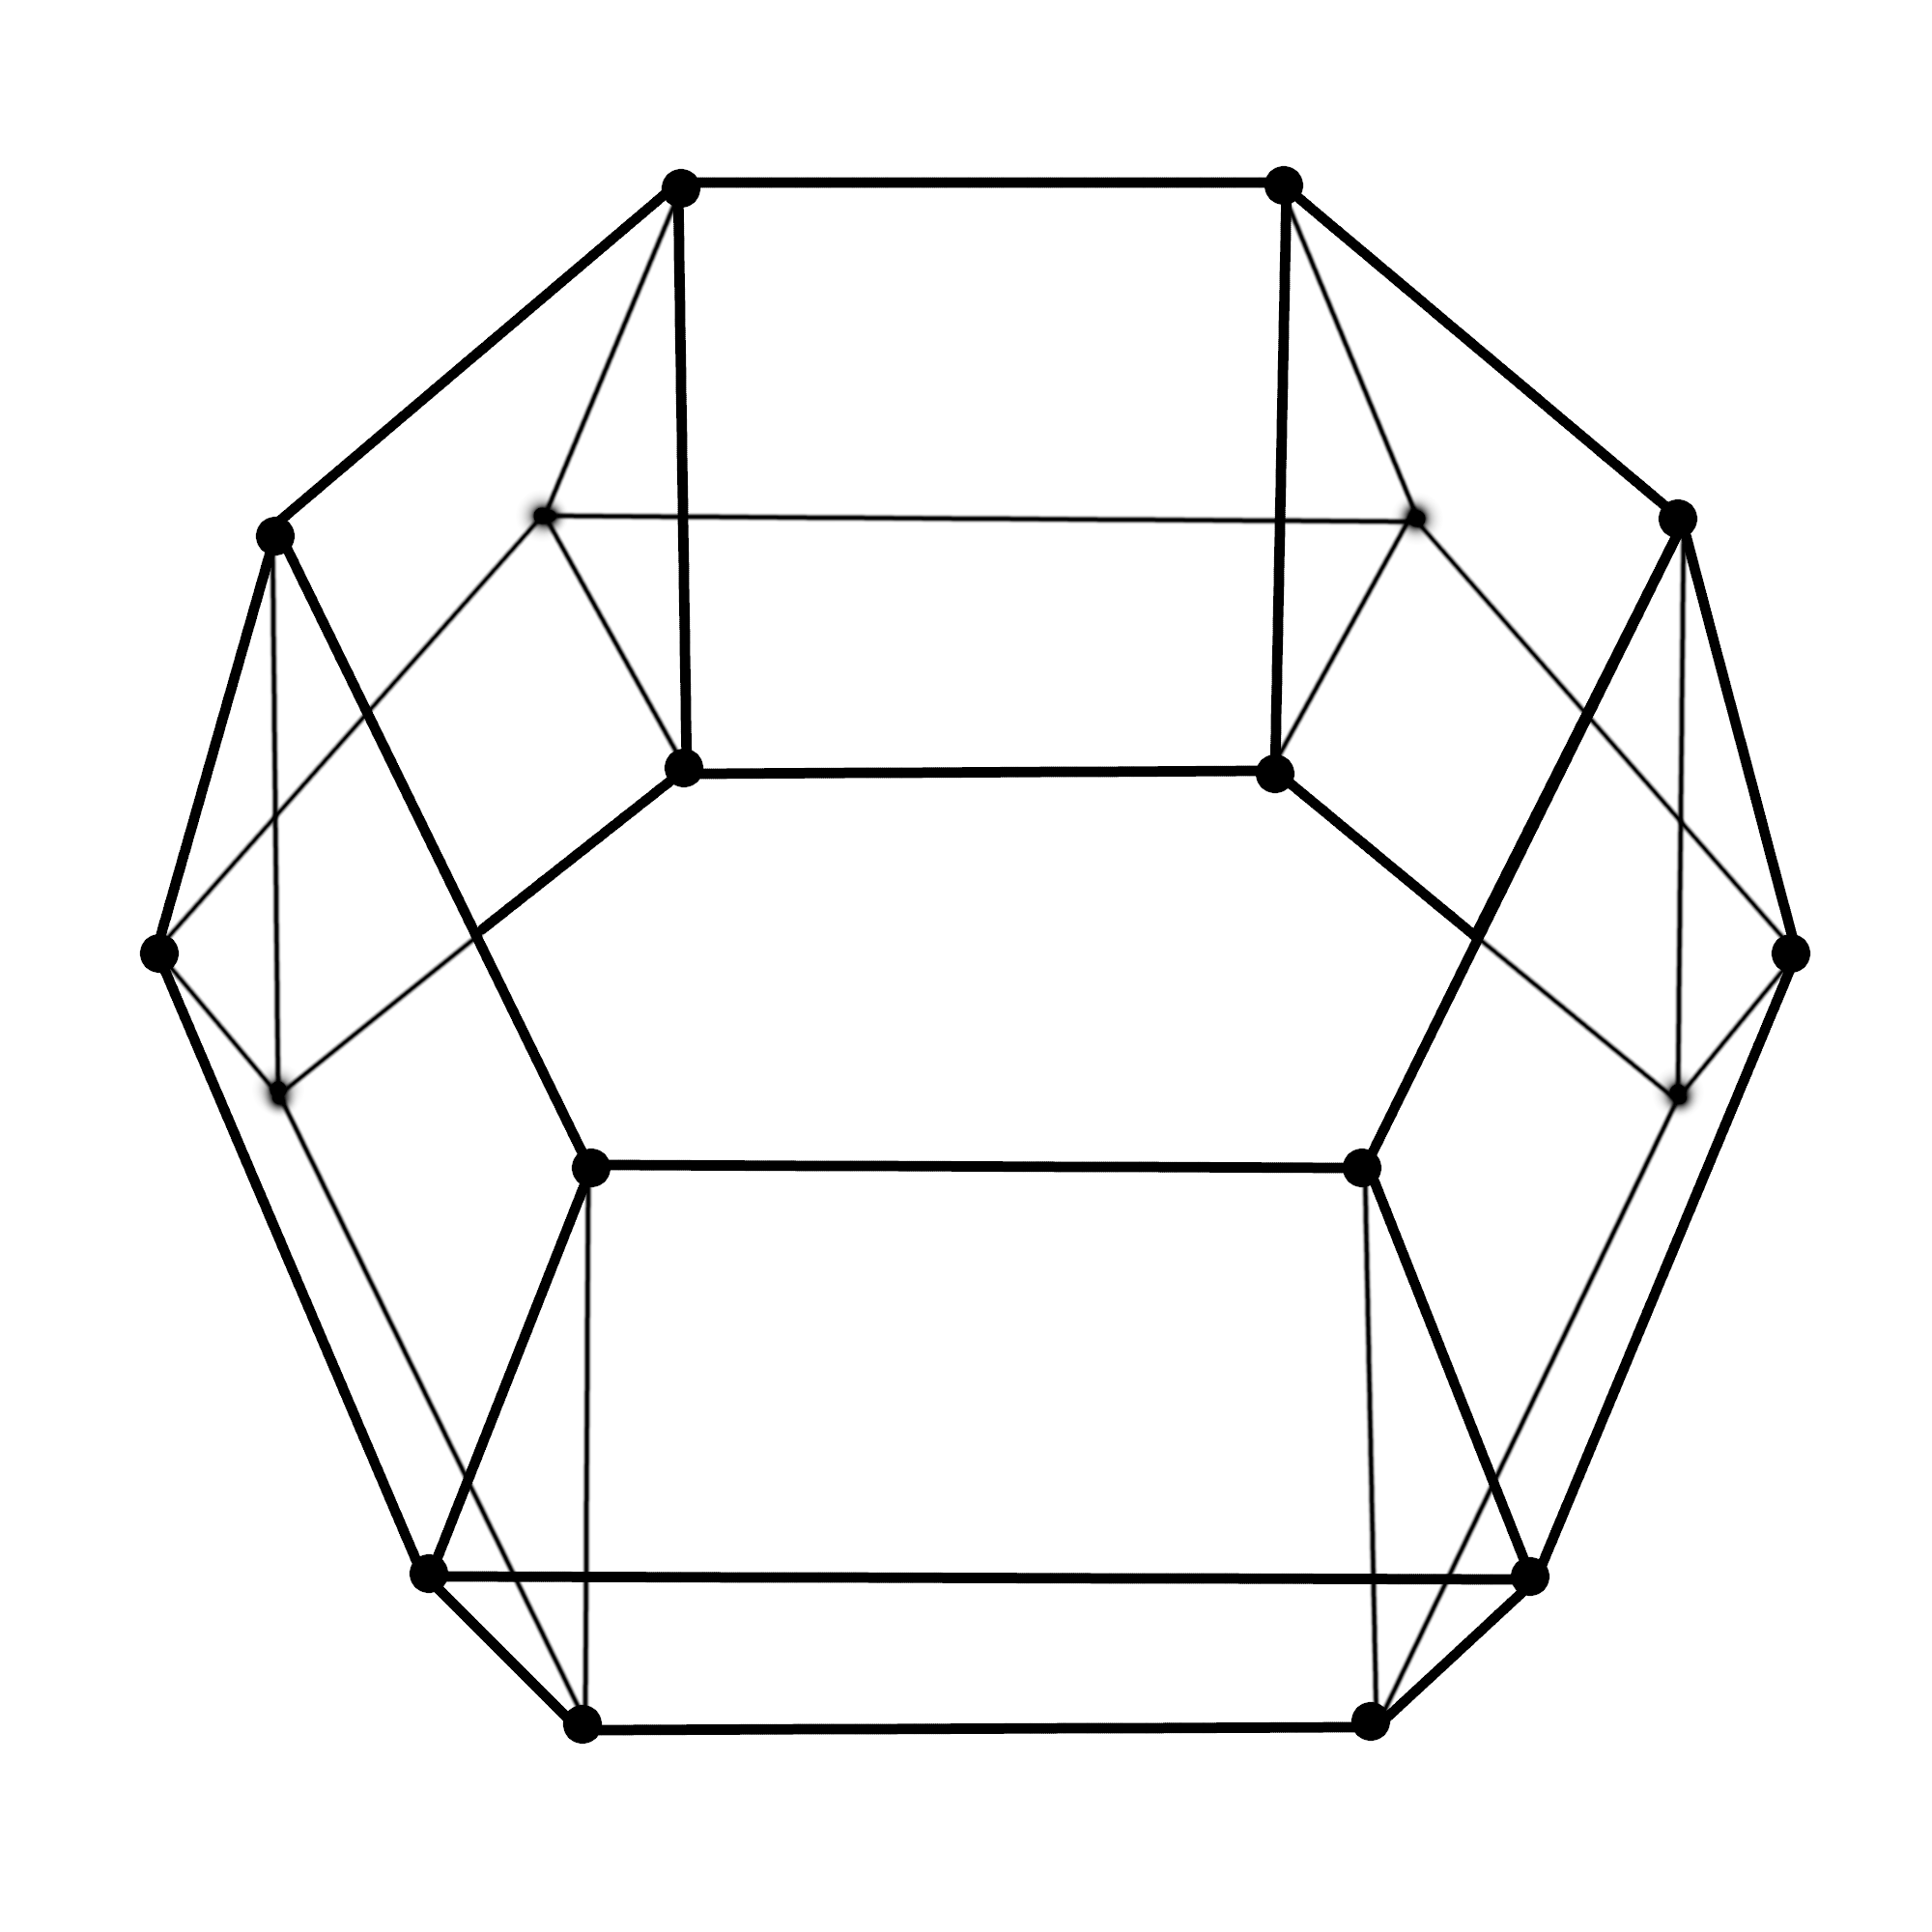
\includegraphics[width=0.25\textwidth]{C3xC6_3.png}
 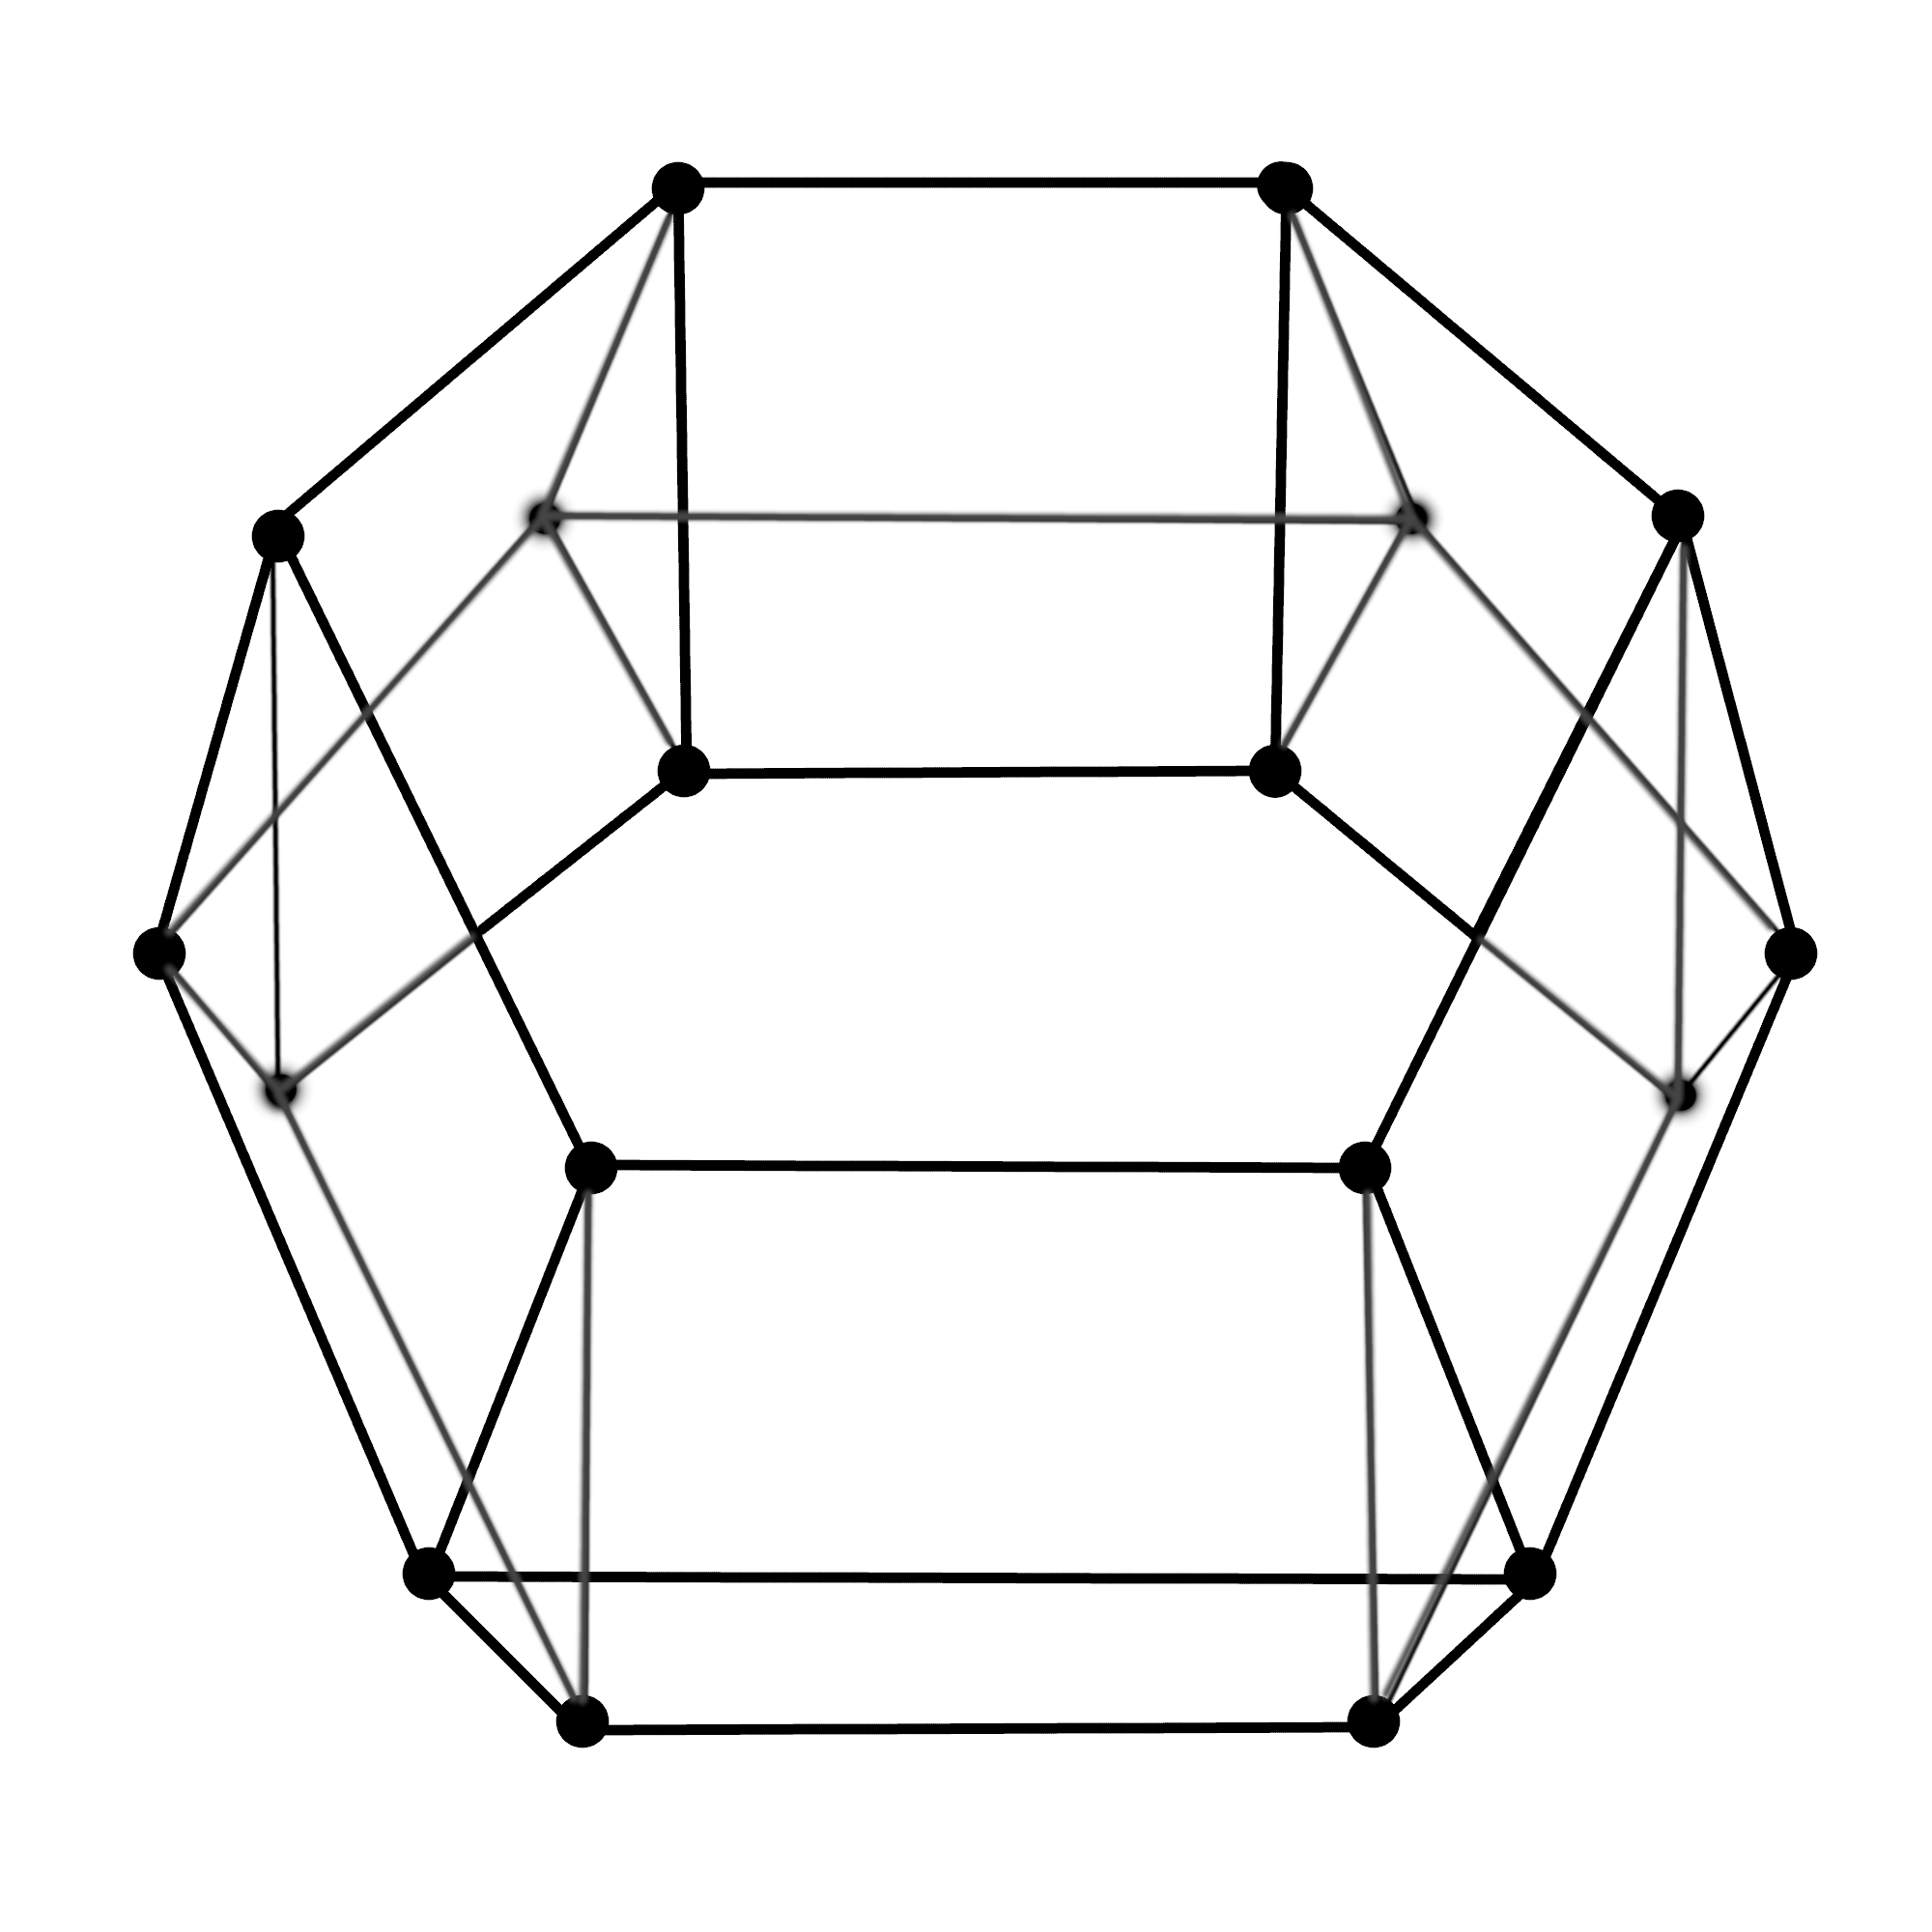
\includegraphics[width=0.25\textwidth]{C3xC6_4.png}
 \caption{$T_{3,6}$}
 \label{c3xc6} %caption vor label unbedingt
\end{figure}
\begin{Bsps}[Torus-Graph]
kreis und Kreis
\end{Bsps}
\todo[inline, color=red]{Lattice Graph ist wieder Mehrdeutig, Gittergraph hier falsch}
\begin{figure}[H]
  \centering
 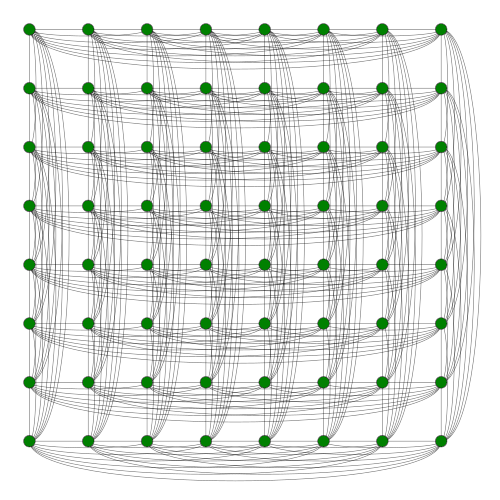
\includegraphics[width=0.5\textwidth]{Rook's_graph.png}
 \caption*{Rooks-Graph $K_8\times K_8$ \\ \tiny{Quelle: \url{https://commons.wikimedia.org/wiki/File:Rook\%27s_graph.svg}}}
 \label{rook} %caption vor label unbedingt
\end{figure}
\begin{Bsps}[kartesisches Produkt von vollständigen Graphen]
%z.B. rooks graph
\end{Bsps}
\todo[inline]{Bei den Beispielen werden wir vollstänige Graphen nutzen, da muss noch kurz argumentiert werden wie da die Eigenwerte sind}
